\documentclass{beamer}

\usepackage[french]{babel}
\usepackage[T1]{fontenc}
\usepackage[utf8]{inputenc}

\usetheme{Warsaw}
\useoutertheme{infolines}

\usepackage{amsmath}
\usepackage{amssymb}
\usepackage{amsthm}
\usepackage{stmaryrd}

\usepackage{listings}
\usepackage{color}

\definecolor{mygreen}{rgb}{0,0.6,0}
\definecolor{mygray}{rgb}{0.5,0.5,0.5}
\definecolor{mymauve}{rgb}{0.58,0,0.82}

\lstset{ %
  backgroundcolor=\color{white},   % choose the background color
  basicstyle=\footnotesize,        % size of fonts used for the code
  breaklines=true,                 % automatic line breaking only at whitespace
  captionpos=b,                    % sets the caption-position to bottom
  commentstyle=\color{mygreen},    % comment style
  escapeinside={\%*}{*)},          % if you want to add LaTeX within your code
  keywordstyle=\color{blue},       % keyword style
  stringstyle=\color{mymauve},     % string literal style
}

\lstset{language=java} 

\usepackage[all]{xy}

%Les sous listes on des triangles
\setbeamertemplate{itemize item}[circle]
\setbeamertemplate{itemize subitem}[triangle]
%Les elements caché sont grisé
\beamertemplatetransparentcovered

\begin{document}

\title{Android - Les Widgets}
\author{Jérémy S. Cochoy}
\institute{INRIA Paris-Saclay | jeremy.cochoy@u-psud.fr}
\date{Novembre 2015}


\begin{frame}
\titlepage
\end{frame}

\begin{frame}
  \begin{columns}[t]
  \begin{column}{5cm}
  \tableofcontents[sections={1-3}]
  \end{column}
  \begin{column}{5cm}
  \tableofcontents[sections={4-8}]
  \end{column}
  \end{columns}
\end{frame}

\begin{frame}
\frametitle{La documentation}

\begin{block}{Votre nouveau livre de chevet.}
\begin{center}
\emph{https://developer.android.com/guide/index.html}
\end{center}
\end{block}

\end{frame}

\section{Le design}

\begin{frame}
\frametitle{Les types de widgets}
\begin{block}{Les différentes catégories de widgets sont :}
\begin{itemize}
\item Informations
\item Collection
\item Contrôle
\item Hybride
\end{itemize}
\end{block}
\end{frame}

\begin{frame}
\frametitle{Widgets d'information}
\begin{center}
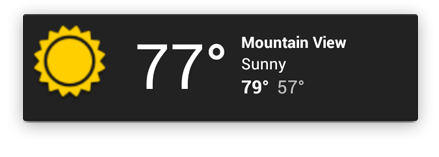
\includegraphics[scale=0.3]{widgets_info.png}
\end{center}

Ces widgets servent à afficher des informations utiles à l'utilisateur, et suivent leur évolution au cours du temps. De bons exemples sont les widgets météo, les horloges, les traqueurs de résultats sportifs...
\end{frame}

\begin{frame}
\frametitle{Widgets de collections}
\begin{center}
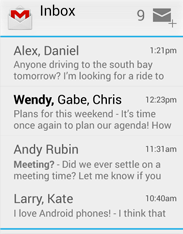
\includegraphics[scale=0.4]{widgets_collection_gmail.png}
\end{center}

Ils sont spécialisés dans l'affichage de collections d'éléments d'un même type, comme des collections d'e-mail, de messages, d'images ou encore d’articles. Ces widgets se concentrent sur deux opérations : parcourir la collection, et ouvrir un élément de la collection pour visualiser l'information complète (contenu d'un e-mail).
\end{frame}

\begin{frame}
\frametitle{Widgets de contrôle}
\begin{center}
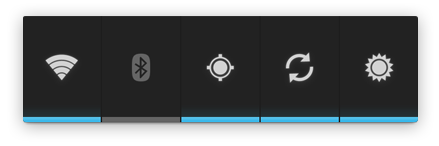
\includegraphics[scale=0.4]{widgets_control.png}
\end{center}

Le but des widgets de contrôle est de permettre l'utilisation rapide d'une fonction très utilisé depuis l'écran d'acceuil, sans avoir besoin de lancer une application. Un exemple typique proviens des lecteurs de musique, qui proposent de mettre à pause la lecture, ou de passer a la musique suivante, sans devoir ouvrir l'application de lecture.
\end{frame}

\begin{frame}
\frametitle{Widgets hybrides}
\begin{center}
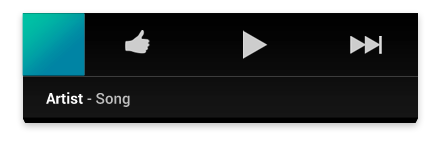
\includegraphics[scale=0.3]{widgets_hybrid.png}
\end{center}

La plupart des widgets rentrent dans une des catégories précédentes, mais il peut arriver que l’emploie de fonctions provenant des différentes catégories soit nécessaire. Dans ce cas, il est recommander de se concentrer sur l'interface sur l'un des types précédent.

\begin{exampleblock}{Un lecteur de musique}
est avant tout un widget de contrôle, mais il permet aussi de suivre le nom du morceau joué, et utilise donc quelques composants d'un widget d'information.
\end{exampleblock}
\end{frame}

\begin{frame}
\frametitle{Mouvements}
\begin{center}
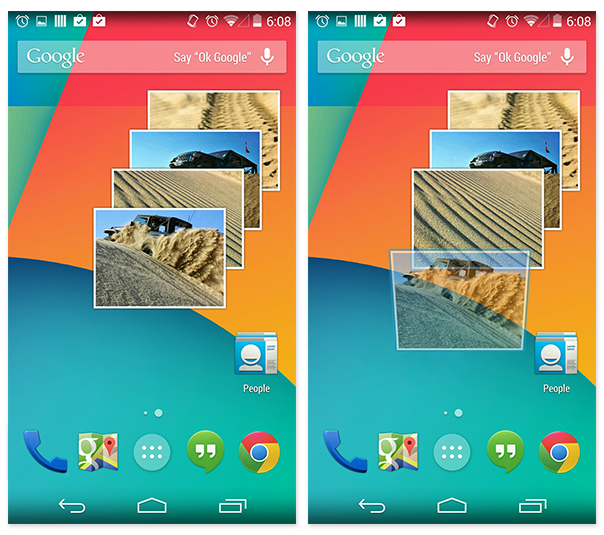
\includegraphics[scale=0.2]{widgets_gestures.png}
\end{center}
Du à leur contexte d'utilisation, les widgets ont des limitations technique sur la façon dont un utilisateur inter-réagira avec. Par exemple, un widget présent sur l'écran d’accueil ne peux accéder qu'aux pressions de l'utilisateur, et au slide vertical. Le slide horizontale est déjà utilisé pour naviguer entre les différents écrans d’accueil.
\end{frame}

\section{Conclusion}

\begin{frame}
\begin{center}
Pour me contacter : jeremy.cochoy@u-psud.fr, merci et à bientôt.

\medskip
\medskip
\medskip
\medskip


\includegraphics[scale=0.18]{android.jpg}
\end{center}
\end{frame}




\end{document}